\section{New Horizons -- Future trends in Ocean Science}
\label{sec:future}

The oceans are changing as a consequence of human activity and yet
because our knowledge about this ecosystem is limited, we cannot
accurately model and predict how it will behave in the future.  The
oceans are vast, occupying almost 71\% of our planet’s surface and yet
less than 10\% of it has been studied. The future of maritime
exploration is therefore heavily dependent on automation and robotics.

The vast variability in spatial and temporal scales that need to be
explored has been a consistent challenge to understand the process and
dynamics on which life on earth depends. Consequently, the use of
automation to replace human presence or even its extension, will
require robotic platforms, a diverse range of sensors and control and
analysis algorithms which can stitch a more incisive picture of the
oceanic environment.
% To do so, it becomes critical to view a patch of the
% ocean across spatial and temporal scales to view processes from the
% large to connect with the small (macro to micro). We believe such a
% patch should be at the meso-scale with coordinated observations
% starting from space based, to aerial, surface and underwater to
% discern the processes in the upper water-column so crucial for our
% understanding of what sustains life on earth.
Further, the absence of a reliable, efficient, and rapid monitoring
system for ocean health is greatly impeding our capacity to respond to
and prevent human-induced threats in a timely, context-relevant and
effective way. This is especially important in coastal regions because
these areas mediate most of the interactions between a significant
percentage of the world population and the oceans.  In addition to
other global forcing, urban population growth has exacerbated
pressures on coastal ecosystems resulting in unhealthy alterations
(e.g., toxic algal blooms, oxygen depletion also referred to as
hypoxia) and deleterious effects on fisheries and human health. These
problems are likely to accelerate in the coming decades as extreme
weather events and storm surges will likely enhance agricultural
pollution runoff and coastal erosion, leading to a worsening coastal
water quality.

\pro (Movable ocEan roboTic obsErvatORy) is conceived as a modular
system with bespoke approaches related to water quality in the world’s
coastal zones.  The fully completed observational system will
constitute both a vertical integration of state-of-the-art hardware
including a small satellite (\smle) constellation, as well as in-situ
air, surface and underwater vehicles, with innovative software and
assimilating ocean models to visualize the information gathered and
predict the near term future, as well as horizontal integration across
disciplines of computer science, marine robotics, engineering, risk
quantification, ocean modeling, and oceanography. The frequent revisit
times over a region that only a constellation of \smle s can provide,
coupled with the latest smart and adaptive AI techniques, will enable
robots to deliver systematic and opportune observations of parameters
relevant to coastal water quality and ocean processes in near
real-time.

Fig. \ref{fig:inverse} visually provides such a perspective. Starting
with the \smle, ocean surface observations can be generated with a
\emph{hyper-synoptic} view of the upper water-column at about 10,000
km\textsuperscript{2} in one snap-shot, with a platform moving in the
order of 15,000 knots, with 'higher' resolution data from
\emph{super-synoptic} UAVs making atmospheric and surface measurements
covering $\sim 1000's$ km\textsuperscript{2} flying at 40--60
knots. Closer in and \emph{in-situ}, potentially synoptic measurements
can be made by ASV's on the surface which can make air/sea flux
measurements, covering potentially $\sim 100's$ km\textsuperscript{2} at
potential 2--10 knots speed. Even higher micro-structure measurements
can then be augmented by AUVs with added in-situ imaging and
water-sampling at the $\sim 10's$ km\textsuperscript{2} scale while
moving through the water column between 1--4 knots. Together this
inverse observational pyramid, forms a cohort of platforms with the
sensors they carry, to detect, track and examine features from space,
all the way to the micro-organisms that inhabit those features.

\begin{figure}[!h]
  \centering
  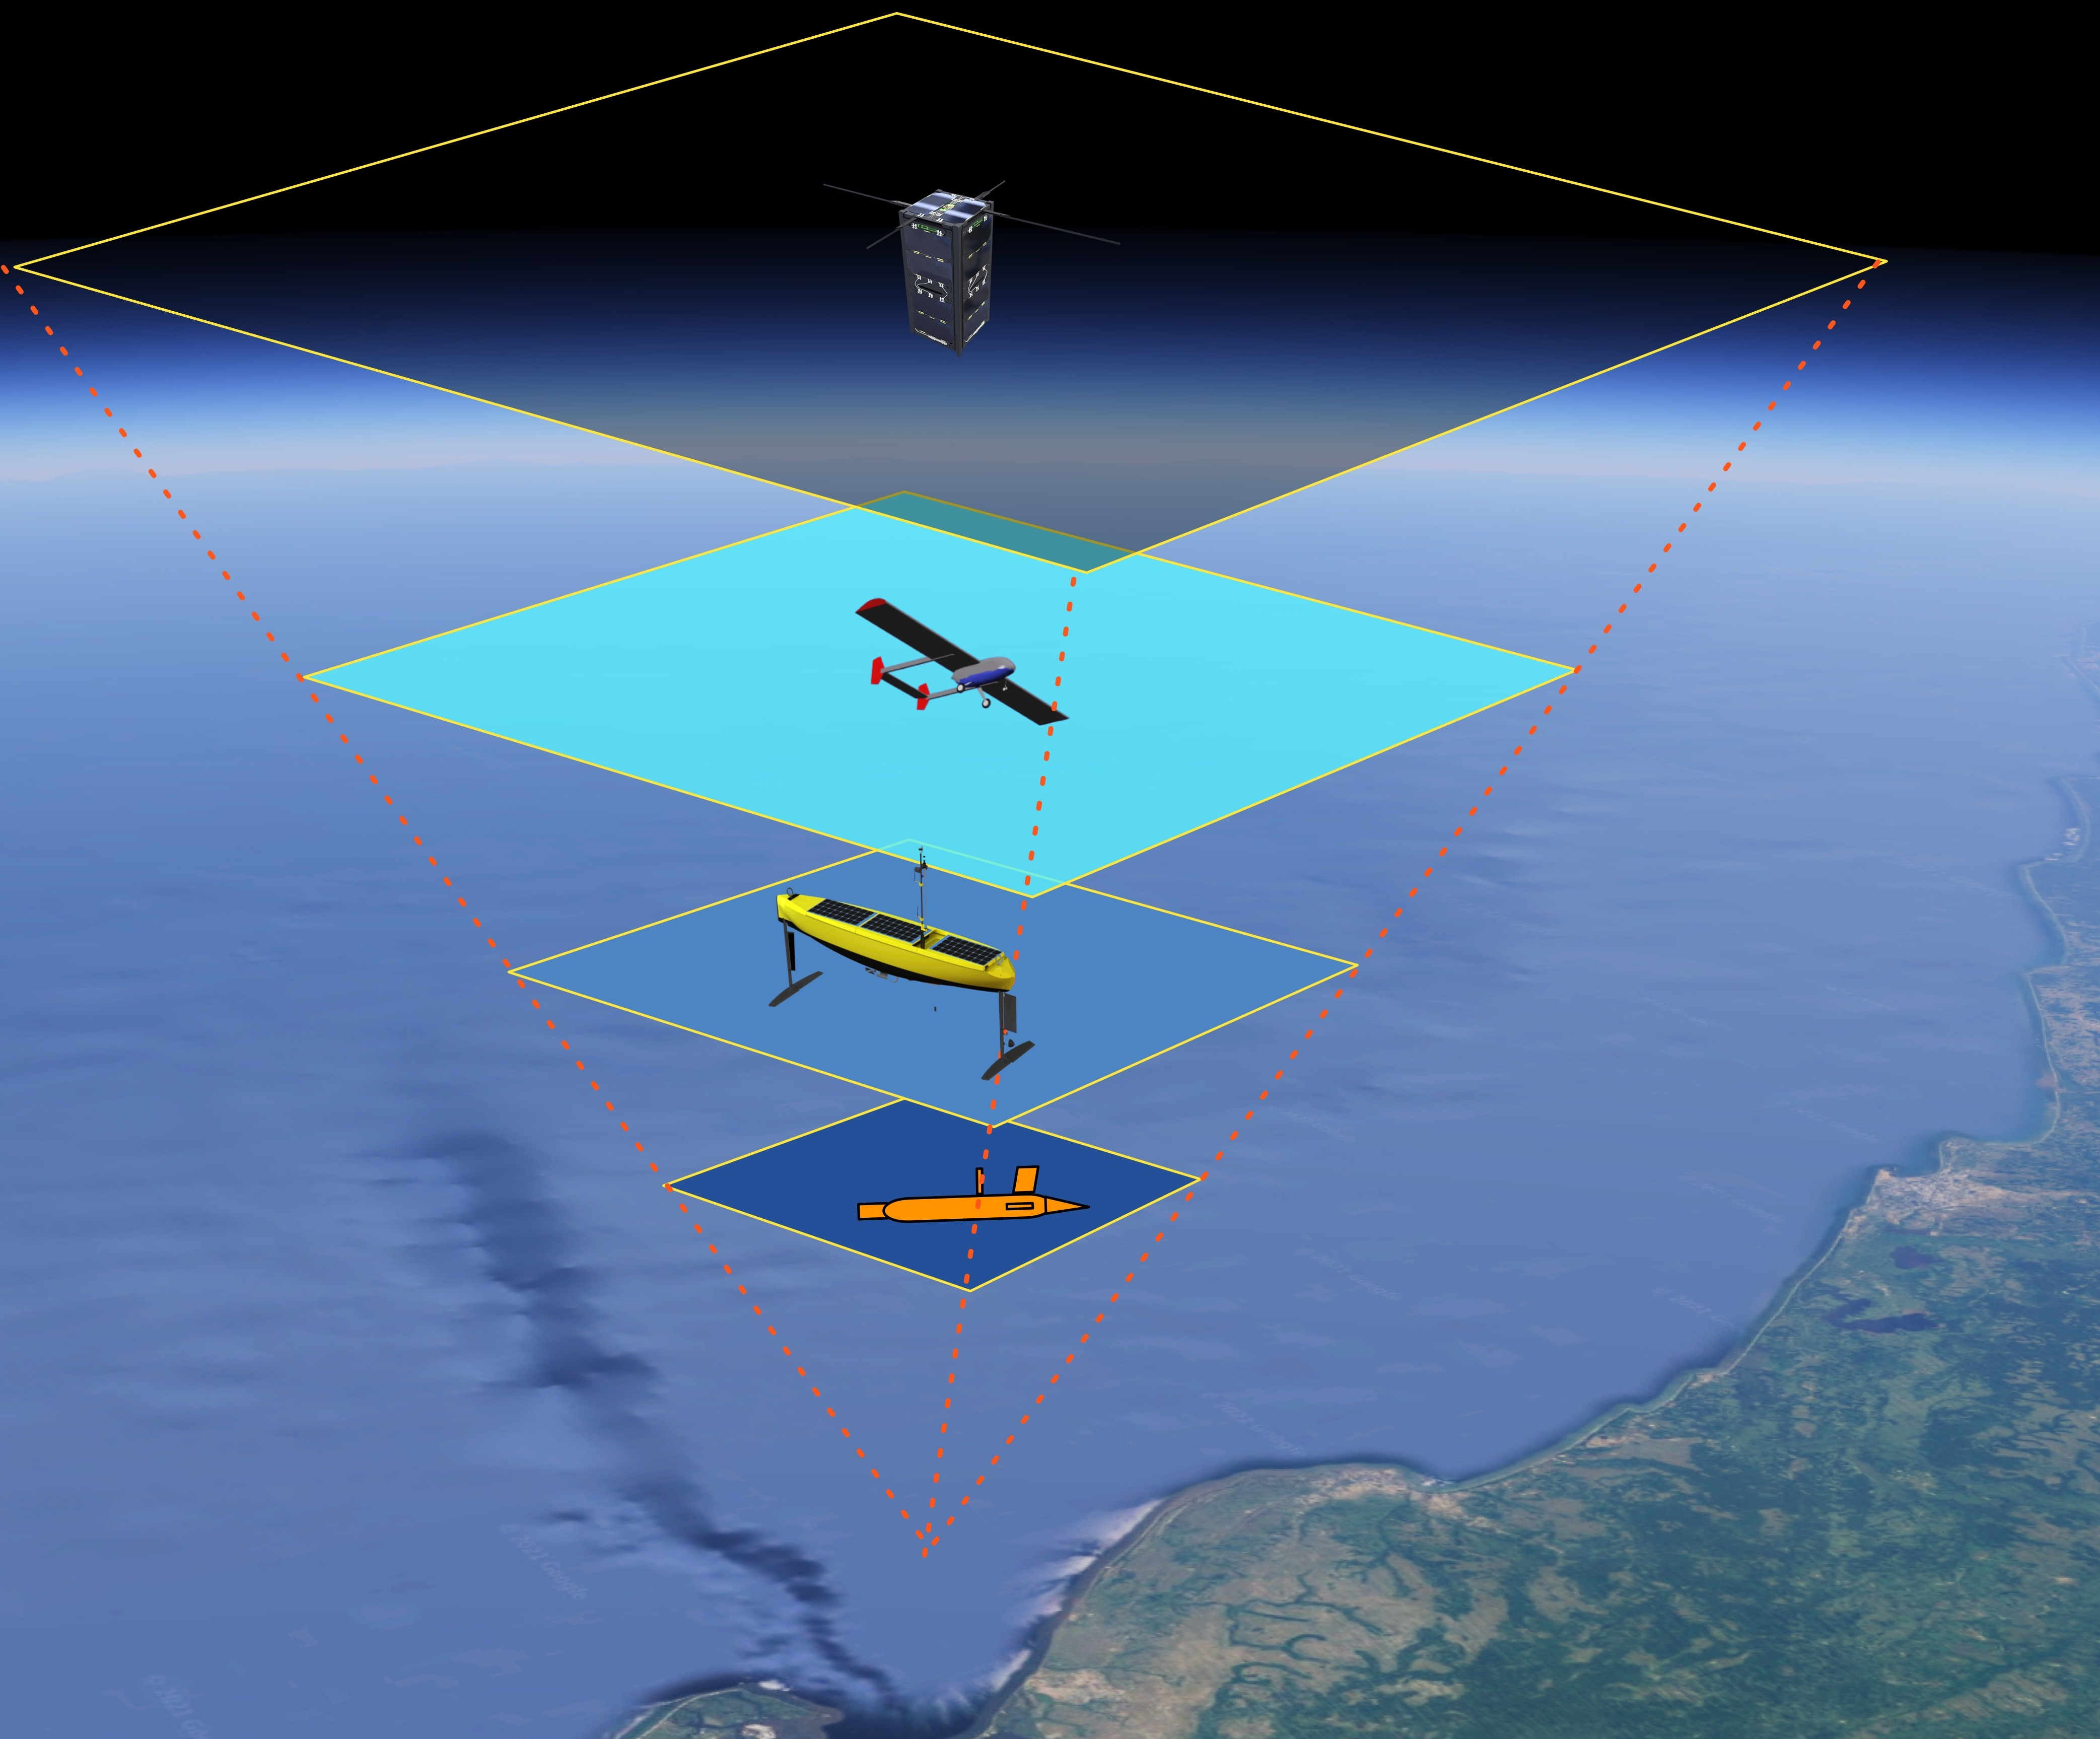
\includegraphics[width=0.9\textwidth]{fig/inverse-pyramid.jpg}
  \caption{Using multi-domain platforms from space, aerial, surface
    and underwater vehicles to observe a patch of the coastal ocean is
    critical to how we can make measurements across the variability in
    spatial and temporal scales. This \textsf{inverse pyramid of
      observational} capability will provide the necessary means to
    discern the bio-geophysical changes in the upper ocean, key to
    human life on Earth.}
  \label{fig:inverse}
\end{figure}

Each platform brings a range of capabilities, from observing at very
large spatial scales via space remote sensing, to making fine scale
measurements in the water column at far slower speeds with AUVs
in-situ. Coordination of these platforms is not necessarily about
managing swarming \cite{osterloh12,lodovisi18,zereik18} or optimal
control behaviors \cite{eichhorn15}, but more about ensuring that
measurements can be made at approximately the region/area/volume in as
adaptive way as necessary. The expense of operating such platforms can
then work in a dynamic that allows for a gradated response which use
(space or aerial) remote sensing to spot a feature of interest, which
then result in an 'event response' situation, which can bring to bear
less expensive in-situ assets like ASVs and AUVs. Aerial platforms can
then be used to scour a larger surface area and direct the deployment
of slower moving ASVs and AUVs in targeted areas. These platforms in
turn, can then use onboard adaptive control to further refine their
observations to generate the necessary fine-scale measurements that
science requires at high-resolution.

The case for \smle 's is equally persuasive. They not only enable
rapid design with miniaturization at affordable cost, while retaining
functional simplicity to implement a space mission, but their lead
time is significantly shorter to more traditional space platforms from
national or trans-national agencies. A \sml can be designed, built and
flown in about 2 years. While the resolution of the data might not be
at the same level as legacy space assets, the rapid pace of technology
development in sensors as well as in algorithms, implies that
resolution gaps are not substantial. Equally, for some ocean
phenomenon like fronts, blooms or oil slicks, capturing the spatial
extant with adequate spectrum resolution, while reducing crucial
revisit time to understand temporal variability.



\begin{figure}[!h]
  \centering
  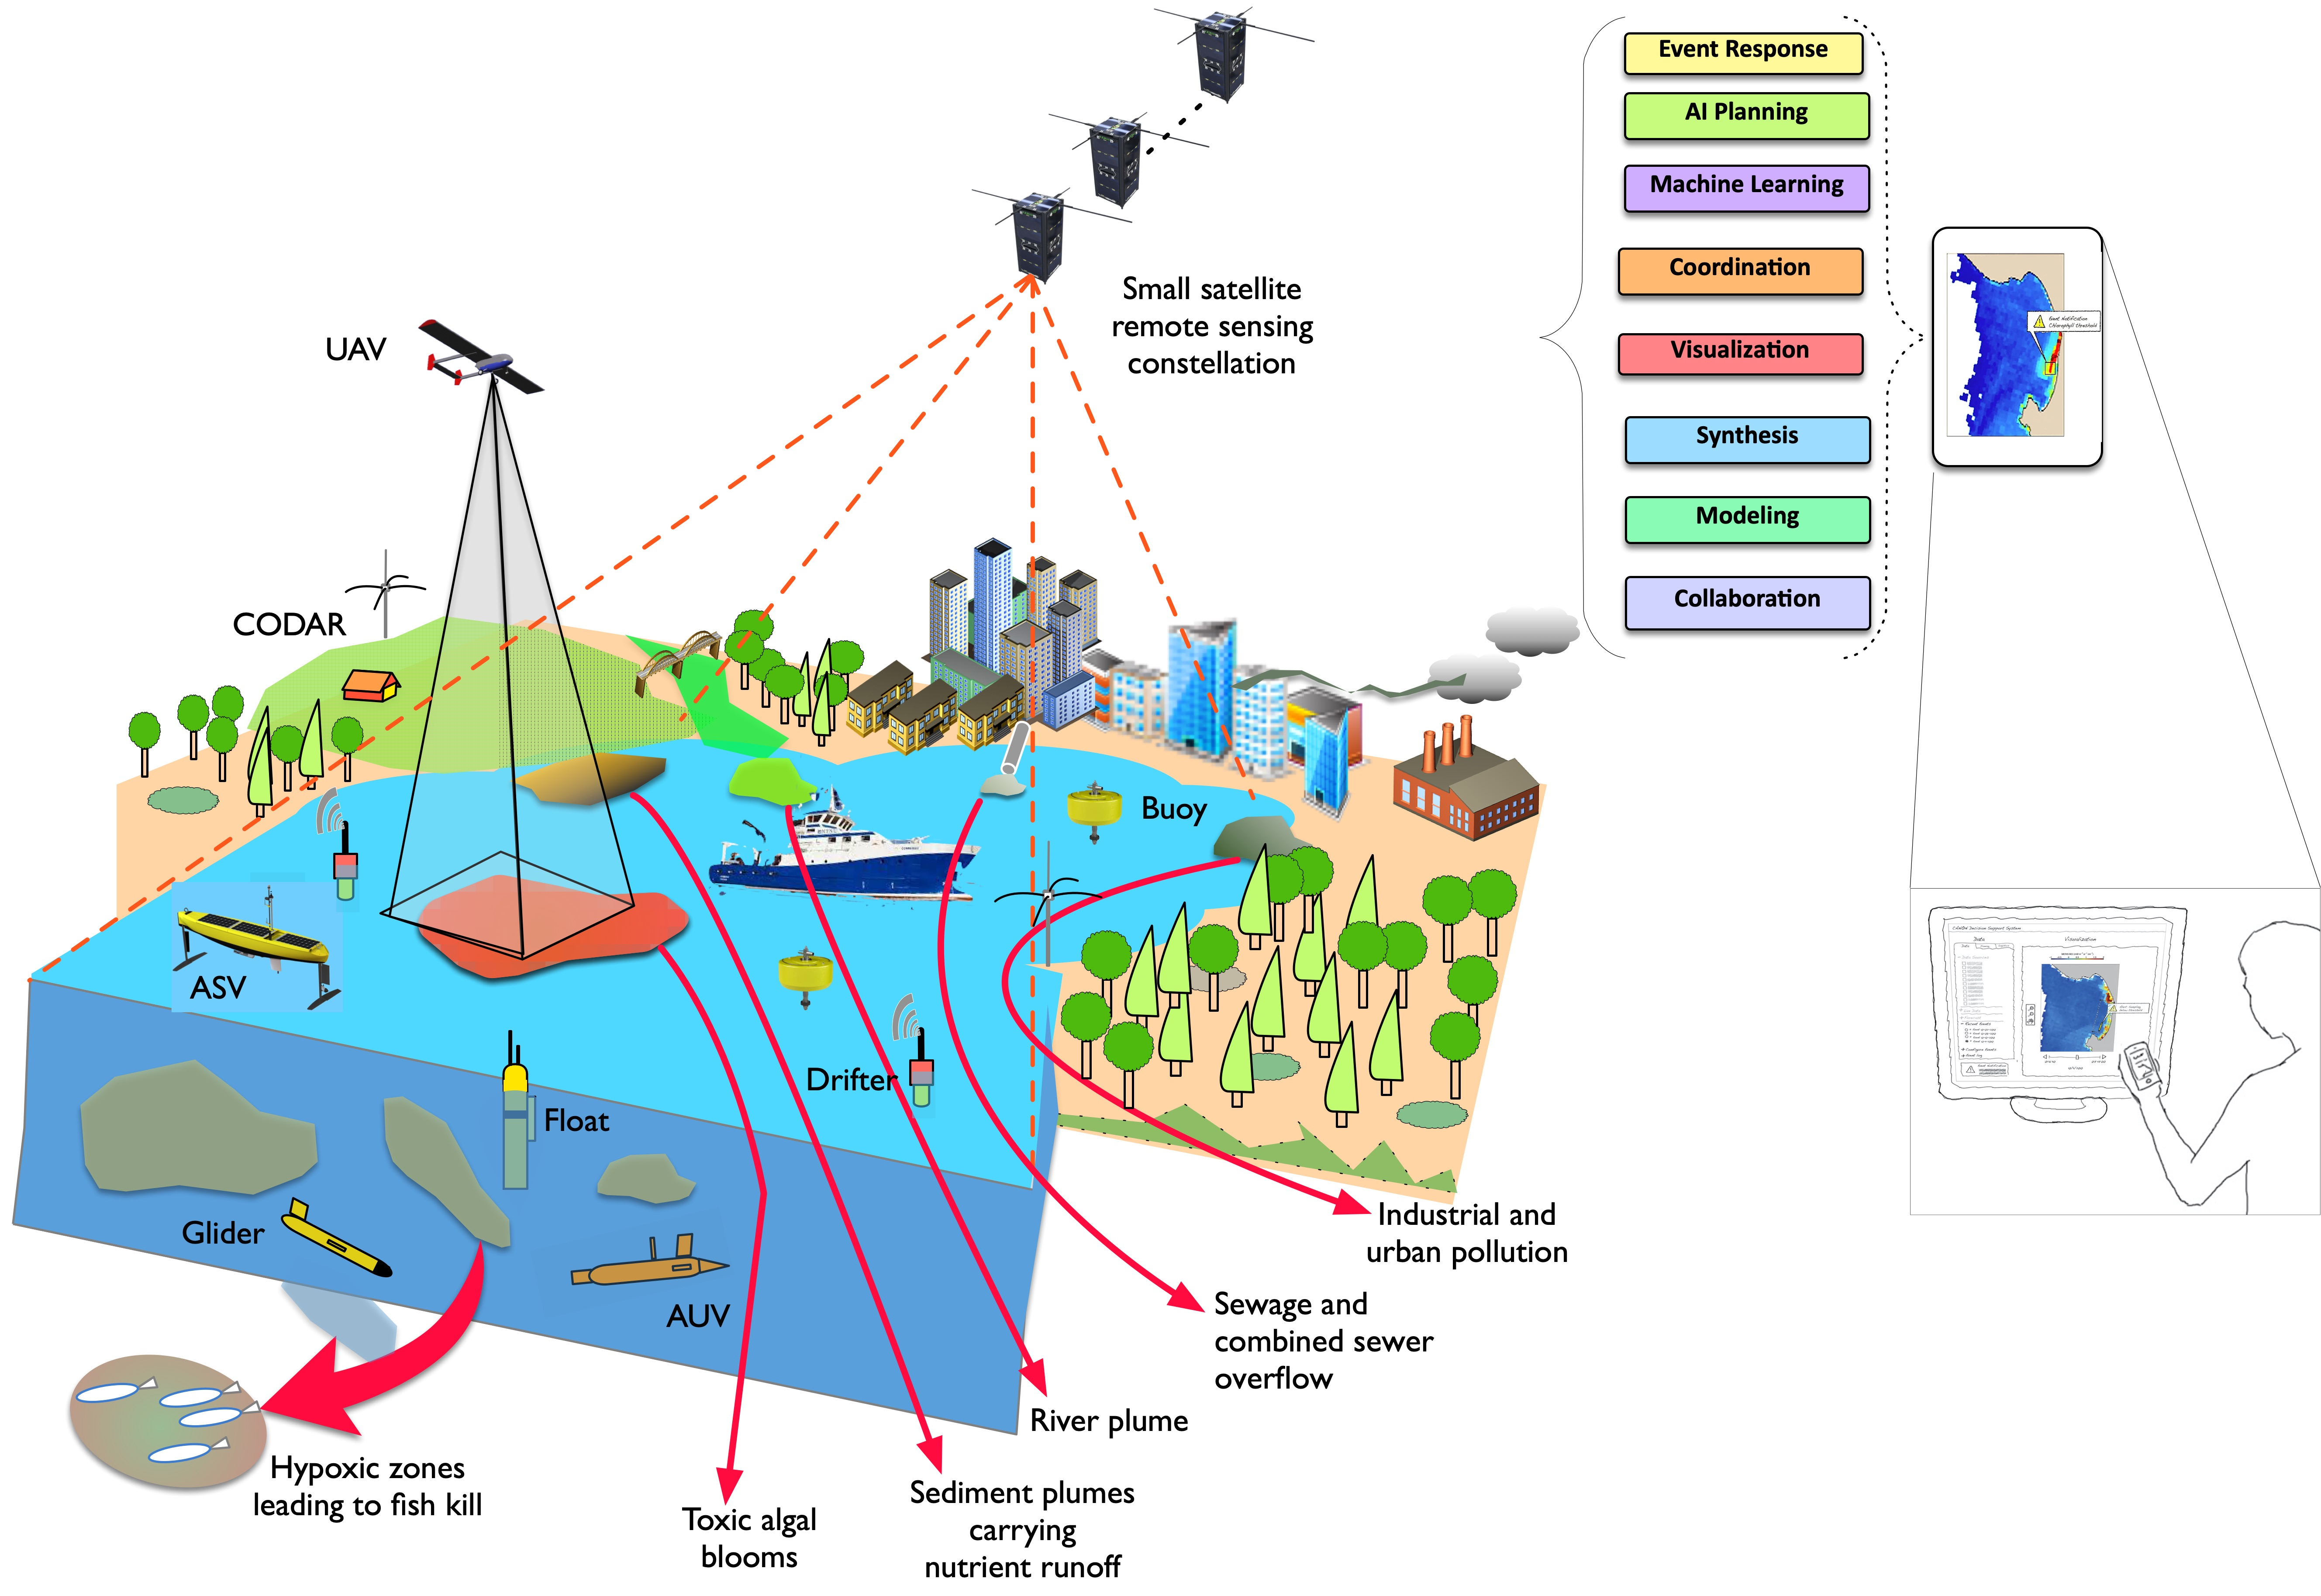
\includegraphics[width=0.9\textwidth]{fig/inverse-pyramid-2.jpg}
  \caption{The backend and embedded computation on robotic vehicles in
  the space, aerial, surface and underwater domains are critical for
  the functioning of the ensemble. The cohort of vehicles will need to
  guided by ocean models, Machine Learned systems to direct them to
  areas of maximal uncertainty, methods to assimilate and fuse data
  from multiple sensors and layered visualization which can show a
  range of possible projections and real-time information.}
  \label{fig:inverse-2}
\end{figure}

This hardware-centric view belies the complexity behind such a likely
scenario since it is backend and embedded software that will actually
provide the necessary means to accomplish the tasks to map dynamic
features in the water-column (Fig. \ref{fig:inverse-2}). Central to
the back end will be data-assimilated ocean models which will
assimilated bio-physical measurements from space and aerial remote
sensing, in addition to digesting continuous measurements from
moorings, buoys, drifters, floats and glider lines to generate
uncertainty maps which can target powered robotic vehicles like ASVs
and AUVs to adaptively sample the water-column in high resolution
\cite{berget18,fossum18,fossum18b,fossum19b,fossum21}.

The AI revolution as noted (Section \ref{sec:ai}) has augmented the
decision-making capacity of marine robotic vehicles in a number of
ways. First, using logic based methods for computational search and
knowledge representation, at the heart of AI, for intelligent
decision-making \cite{ryan10,fossum18,fossum18b}, curiosity driven
exploration \cite{girdhar14}, statistical pattern matching and machine
learning of models of spatial and temporal variability of
environmental variables \cite{fossum19b}.

We consider ``Artificial Intelligence'' to be the broader field, not
to be confused with what is clearly Machine Learning (ML), the latter
related to understanding patterns in acquired data and fitting it to
what a robotic vehicle is observing in-situ; we will therefore
separate out the implications of AI and ML. In \proe, we will use
methods in automated decision-making and autonomous control to
intelligently sample in space and time \cite{graham12}. Typical
methods in sampling deal with static sensors making measurements in
static fields (such as ponds) or static sensors in dynamic fields
(such as buoys in the coastal ocean). To enable mobile (or dynamic)
sensors on robotic platforms measuring dynamic fields requires
intelligent control driven by Sampling algorithms. For instance,
measuring sub-surface chlorophyl max (SCM's) which feed a surface
bloom and characterizing it over space and time, requires algorithmic
methods such as Gaussian Processes \cite{fossum18}. This method
applies well in multi-variate fields, where spatially relevant data
with an \emph{apriori} estimation are available, and estimates
internal to this field are needed to be filled. Such a statistical
measure of estimation is well suited to a mobile robot that can use
estimates from, say, remote sensing to close the uncertainty gap
within a dynamic field, such as a bloom, need to be sampled. To do so
then, the robot needs to be guided reactively, within regions of
statistical uncertainty to update the 'known unknowns', something an
AI-based decision-making system can do. In so doing, the
decision-making 'AI' keeps the larger context of a complex goal,
e.g. surveying a volume of water, while greedily evaluating and
constructing the distribution of one or more variables in order to
construct the dynamically varying field. An important assumption of
stationarity is the dynamism of the field itself; typically in the
upper water column coastal or open oligotrophic ocean, the field
varies slowly ($< 5$ m/sec) and the applicability of such methods has
proven to be viable. The AI, therefore is to balance the needs of the
\emph{deliberative} or longer term goals of a robot, with its more
\emph{reactive} responses. In \proe, such a system will be fielded
embedded on a robot to make such trades to demonstrate
'intelligence' \cite{fossum18,fossum18b}.

Given the spatial and temporal spread of upper water column processes
from sub-centimeter scales to tens of kms (Fig. \ref{fig:platforms2}),
methods to capture the dynamics of a biological fields need to rely on
a mix of algorithmic approaches.



% This could be the core of the m/s -- a look ahead to what we think the
% contributions of AI and Robotics can do, leveraging networked vehicle
% technologies, given large spatial extents to be sampled. 

\begin{enumerate} 
\kc{
% \item Implications of the use of robotic vehicles -- plusses and
%   challenges. The role of vehicles in space, aerial, surface and
%   underwater environments

% \item how new generations of spacecraft (incl. SmallSats) could alter
%   the landscape — e.g. our pitch to Audacious
  
\item How AI/ML can tie the needs of observational requirements and
  alleviate the issue of space/time and understanding spatio-temporal
  cause-effect relationships

\item The use of robots in security and surveillance. Legal implications
  related to use of robotic vehicles in such domains. 
}
\end{enumerate}

